\chapter{Closed Boundary Motion}
\label{chap:closedboundary}

\lettrine{A}{n} interesting case of study for understanding mathematical and numerical aspects of grain growth simulation is to understand the growth of a closed boundary which tries to minimize its energy. Let $\vxi(s,t) = \langle x(s,t), y(s,t)\rangle,\, s \in [0, 2\pi]$ a closed curve in $\Reals^2$ such that $\vxi(0,t) = \vxi(2\pi,t)$, where $s$ is the parametrization variable and $t$ is the time variable. This will be the base definition of a closed boundary. Let $\mylvec(s,t) = \dxids(s,t)$ a tangent vector to the boundary $\vxi$ and $\T(s,t) = \unitl$ the unit tangent vector in the same direction. Also let $\N(s,t) = \dTds(s,t)$ a unit normal vector to $\vxi$. From the total energy equation in \eqref{eq:energy}, the energy of this boundary becomes a single integral term:
\begin{equation}
    E(t) = \int_0^{2\pi} \norm{\mylvec(s,t)}\, ds,
    \label{eq:energyclosed}
\end{equation}
where for simplicity we assumed an isotropic regime, \ie $\gamma = 1$. Taking the derivative of \eqref{eq:energyclosed} with respect to the time yields:
\begin{equation}
    \dfrac{dE}{dt}(t) = \int_0^{2\pi} \unitl \cdot \dlvecdt(s,t) \, ds.
    \label{eq:dEdtclosed}
\end{equation}
Let $\vel(s,t) = \dxidt(s,t)$ the velocity of the boundary. Equation $\eqref{eq:dEdtclosed}$ becomes:
\begin{equation}
    \dfrac{dE}{dt}(t) = \int_0^{2\pi} \T(s,t) \cdot \dvds(s,t) \, ds.
    \label{eq:dEdtclosed2}
\end{equation}
Integrating by parts \eqref{eq:dEdtclosed2} we obtain:
\begin{align}
    \dfrac{dE}{dt}(t) &= \T(s,t)\cdot\vel(s,t)\eval{0}{2\pi} - \int_0^{2\pi}  \dTds(s,t) \cdot \vel(s,t) \, ds \nonumber\\
    &= -\int_0^{2\pi} \dTds(s,t) \cdot \vel(s,t)\, ds. \label{eq:dEdtclosed3}
\end{align}
Thus, we will use \eqref{eq:dEdtclosed3} to understand the motion of a closed boundary.

\section{Curvature based motion}

Curvature based grain growth models assumes that the velocity of the boundaries is in the direction of its normal vector and proportional to its curvature $\kappa(s,t)$ \cite{Kinderlehrer2006}. Thus the velocity of the boundary can be defined as \cite{thomascalculus}:
\begin{equation}
    \vel(s,t) = \kappa(s,t)\N(s,t). %\label{eq:closedboundaryvelocity}
    \nonumber
\end{equation}
This term can be obtained also from the derivative of the vector $\T$ with respect to the arc length $\AL$:
\begin{align}
    \dTdAL(s,t)  &= \kappa(s,t)\N(s,t) \nonumber\\
    \dTds(s,t) \dsdAL &=\kappa(s,t)\N(s,t). \label{eq:dTdAL}
\end{align}
Let $\AL(s)$ the arc length of the boundary up to $s$, given by:
\begin{equation}
    \AL(s) = \int_0^{s} \norm{\mylvec(s,t)}\, ds,
    \label{eq:arclen}
\end{equation}
then we can obtain $\dsdAL$ from \eqref{eq:arclen} by derivating with respect to $s$ as:
\begin{align*}
    \frac{d\AL}{ds} &= \norm{\mylvec(s,t)} \\
    \frac{ds}{d\AL} &= \frac{1}{\norm{\mylvec(s,t)}}.
\end{align*}
Replacing in \eqref{eq:dTdAL} we obtain:
\begin{equation}
    \dfrac{1}{\norm{\mylvec(s,t)}} \dTds(s,t) = \kappa(s,t)\N(s,t).
    \label{eq:curvresult}
\end{equation}
Therefore to obtain curvature based motion we need to compute the grain boundary velocity as:
\begin{equation} \vel(s,t) = \frac{1}{\norm{\mylvec(s,t)}}\dTds(s,t). \label{eq:curvvelocity}
\end{equation}

\section{Coupled model based motion}

Let's consider the same boundary parametrization as the coupled model from \eqref{eq:boundarydiscret}. We do not need to handle a special treatment of vertices and interior points.  Since we are dealing with a periodic condition for this grain boundary, instead of classic Lagrange interpolator functions $\phi_i$, we should use another interpolation basis, for example the periodic sinc interpolator \cite{trefethen2000spectral}. The velocity of the boundary $\vel$ is expressed in terms of the parametrization as:
\begin{equation}
    \vel(s,t) = \velboundary.
\end{equation}
We can replace the velocity term in \eqref{eq:dEdtclosed3} to obtain the derivative of the energy in terms of the boundary.
\begin{align}
    \dfrac{dE}{dt}(t)
    &= -\int_0^{2\pi} \dTds(s,t) \cdot \left( \velboundary \right)\, ds \nonumber \\
    &= -\sum_{i=1}^{n}  \dotx[i](t) \cdot \int_0^{2\pi}  \dTds(s,t) \phii{i}{s}\, ds.
    \label{eq:dEdtboundclose}
\end{align}
The velocity at the boundary points $\x[i]$ can be defined from \eqref{eq:dEdtboundclose} such that decreases the energy of the grain system as:
\begin{equation}
    \dotx[i](t)= \frac{\zeta}{\norm{\mylvec(s_i,t)}}\int_0^{2\pi}  \dTds(s,t) \phii{i}{s}\, ds,
    \label{eq:coupledvelocity}
\end{equation}
%
where we introduced the curvature term from \eqref{eq:curvresult} for each discrete boundary point and a constant $\zeta$ which depends on the specific parametrization and interpolation and will be defined in the next section. This evolution equation contrasts with the curvature based evolution equation found before. Here we have instead of a normal vector at a given point an integral along the boundary. In order to find more agreement with the curvature based equation, we can study a circular boundary which holds simple formulas.

%The following sections shows the theoretical evolution of a circular boundary and how the discrete boundary equations successfully approaches the evolution. This result can be extended to general boundary shapes, whilst the theoretical ratios are not derived in the later, a generic boundary evolving and minimizing energy reaches a state where becomes a circle, and thus the prior results are again valid.

\subsection{Circular Boundary}
\label{sec:circularboundary}

This simple case is very illustrative, since we can obtain an explicit formula for $\dfrac{dE}{dt}$ and also the area rate of change $\dfrac{dA}{dt}$ . First we describe analytic results for boundary evolution and then we apply the coupled model idea of interpolate the boundary and obtain new equations.

The equation that describes this boundary is:
\begin{equation}
    \vxi(s,t) = R(t)\langle \cos(s), \sin(s) \rangle,\quad R(t) > 0 \;\;\forall\,t \geq 0,
    \label{eq:circle}
\end{equation}
where we have decoupled the spatial parametrization in polar coordinates with the radial time-dependence. Notice that $\norm{\vxi(s,t)} = R(t)$, that is, for a fixed time $t=\tau$, the boundary preserves a constant radius and thus constant curvature along the boundary. The tangent vector $\mylvec(s,t)$ is nothing but:
\begin{equation*}
    \mylvec(s,t) = R(t)\langle -\sin(s), \cos(s) \rangle,
\end{equation*}
and again its norm $\norm{\mylvec(s,t)} = R(t)$ just like $\vxi$. This implies that the unit tangent vector is:
\begin{equation*}
\T(s,t) = \langle -\sin(s), \cos(s) \rangle,
\end{equation*}
and the normal vector is:
\begin{equation*}
    \dTds(s,t) = \langle -\cos(s), -\sin(s) \rangle,
\end{equation*}
which is a vector always pointing to the circle center. If we took these results and plug them in \eqref{eq:dEdtclosed3} yields:
\begin{equation*}
    \dfrac{dE}{dt}(t) = \int_0^{2\pi}  \langle \cos(s), \sin(s) \rangle \cdot \vel(s,t)\, ds.
\end{equation*}
Considering that the boundary moves proportional to the curvature and in a normal direction, we replace the velocity term with the curvature result in \eqref{eq:curvresult}:
\begin{align}
    \dfrac{dE}{dt}(t) &= \int_0^{2\pi}  \langle \cos(s), \sin(s) \rangle \cdot \frac{1}{\norm{\mylvec(s,t)}} \langle -\cos(s), -\sin(s) \rangle\, ds \nonumber\\
    &= \int_0^{2\pi} -\frac{1}{R(t)} \,ds \nonumber\\
    &= -2\pi \kappa(t) \label{eq:dEdtcircle}
\end{align}

Area rate of change can also be obtained from the definition of area given the boundary parametrization in \eqref{eq:circle}:
\begin{align}
    A(t) &= \frac{1}{2} \int_0^{2\pi} \norm{\vxi(s,t)}^2\, ds\nonumber\\
    \dAdt(t) &= \int_0^{2\pi} \vxi(s,t)\cdot \vel(s,t)\,ds \nonumber\\
    &= \int_0^{2\pi} R(t)\langle \cos(s),\sin(s)\rangle \cdot \frac{1}{R(t)} \langle -\cos(s),-\sin(s)\rangle \,ds \nonumber\\
    &= -2\pi \label{eq:dAdtcircle}
\end{align}
This means that the rate of change for the area of a circle is constant. The evolution of the radius $R(t)$ over time can be explicitly found by comparing the velocity of the curvature in \eqref{eq:curvresult} with the circle velocity expression:
\begin{align}
    \frac{dR}{dt}(t) &= -\frac{1}{R(t)} \label{eq:circvel}\\
    %\frac{1}{2}(R(t)^2 - R(0)^2) &= t \\
    R(t) &= \sqrt{R_0^2 - 2t} \label{eq:radii},
\end{align}
where $R(0) = R_0$ is the initial radius of the circle at time $t=0$. The equation is valid as long as $R_0^2 > 2t$. In the limit, the circle should become a single point, and related vectors becomes indeterminate. Finally, the complete description of a circular boundary is given by:
\begin{equation}
    \vxi(s,t) = \sqrt{R_0^2 - 2t}\,\langle \cos(s), \sin(s) \rangle.
\end{equation}
The coupled model based formula induces a different result from the velocity found in \eqref{eq:circvel}. Assuming equispaced points in $[0, 2\pi]$, we replace $\mylvec$ and $\dTds$ for the circle in \eqref{eq:coupledvelocity} to obtain:
\begin{equation}
    \dotx[i](t) = \frac{1}{R(t)} \int_0^{2\pi}  \langle -\cos(s), -\sin(s)\rangle \,\phi_i(s)\, ds,
\end{equation}
where $\phi$ the periodic $\sinc$ interpolation function. Notice that this definition needs even number of discrete points. If we replace the definition of the periodic $\sinc$ we obtain:
\begin{align}
    \dotx[i](t) &= -\frac{1}{R(t)} \int_0^{2\pi} \left\langle \cos(s)\frac{\sin(\pi(s-s_i) / h)}{\frac{2\pi}{h} \tan((s-s_i)/2)}, \sin(s)\frac{\sin(\pi(s-s_i) / h)}{\frac{2\pi}{h} \tan((s-s_i)/2)} \right\rangle\,ds\\
    &= -\frac{1}{R(t)}  \frac{2\pi}{n}\left\langle\cos \left(\frac{2\pi i}{n}\right), \sin\left(\frac{2\pi i }{n}\right)\right\rangle.
    \label{eq:curvaturevelocity}
\end{align}
Under $\sinc$ interpolant, the constant $\zeta$ from \eqref{eq:coupledvelocity} becomes $2\pi/n$. Figure \ref{fig:circularboundary} shows the evolution of the boundary with 14 points using the velocity equation from \eqref{eq:curvaturevelocity}. The discrete data is extracted from a circle and then is interpolated using the sinc periodic interpolator. For this example we set $R_0 = 2$, which implies that the limit time of the simulation is $t_{lim}=2$. The theoretical description of the circle matches qualitatively with the interpolated curve, and for simplicity of presentation the theoretical circle is not shown. 

\begin{figure}[t]
    \centering
    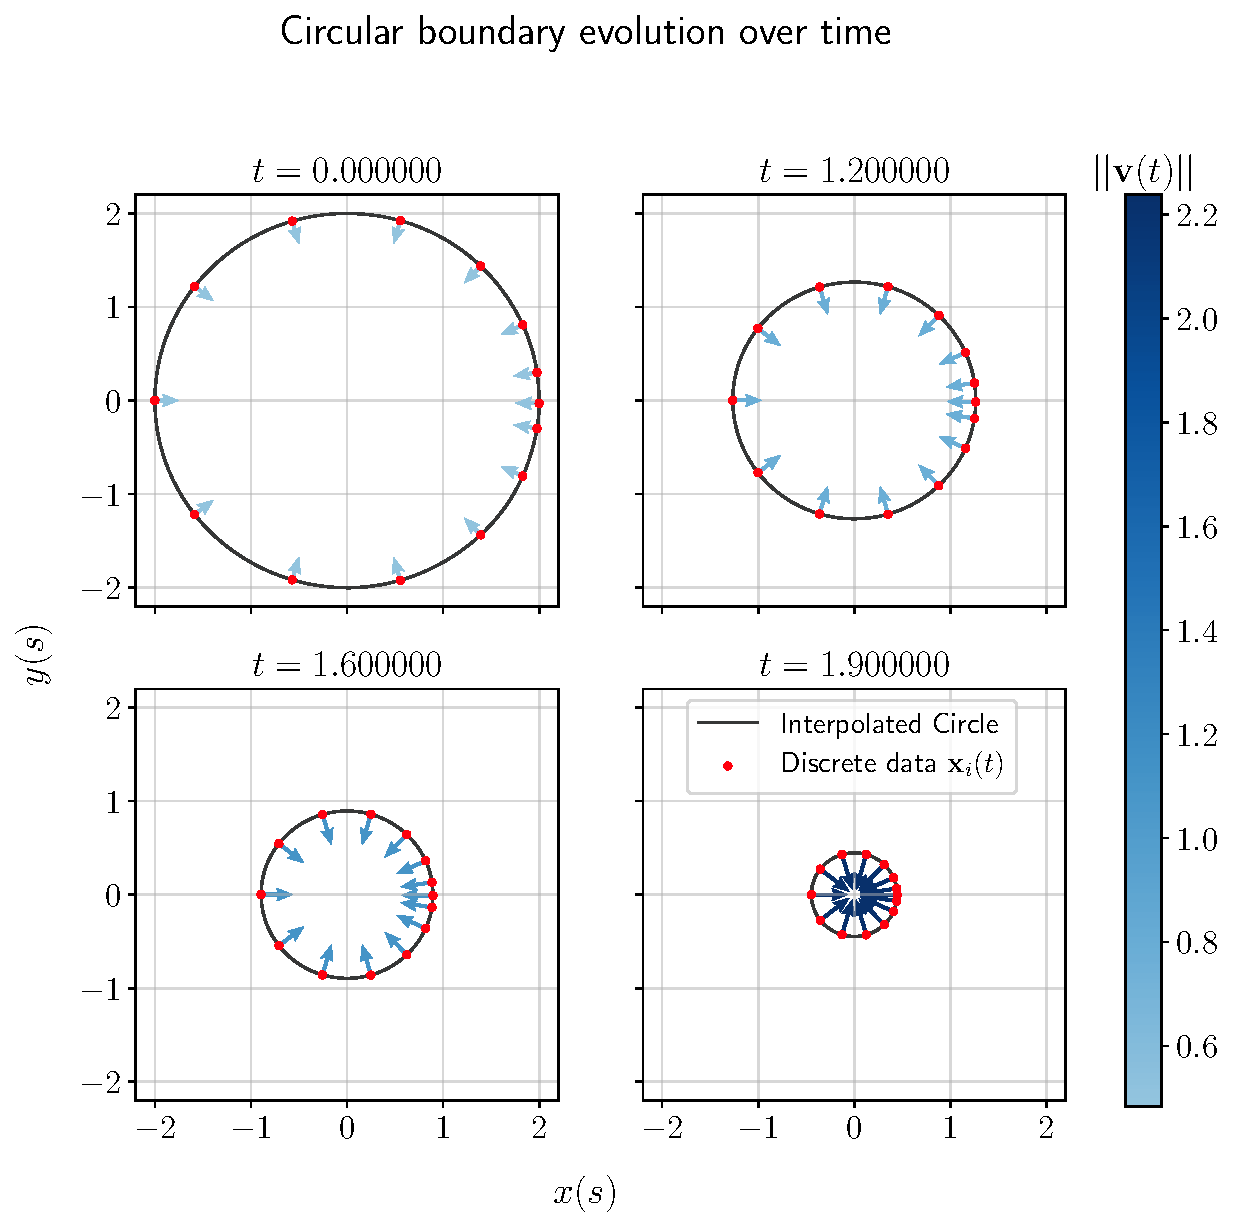
\includegraphics[scale=0.6]{circularboundary.pdf}
    \caption[Circular boundary evolution]{(Top left) The initial condition at $t=0$ of the circular boundary with $R_0 = 2$. (Top right, bottom left) After some time the circle start to shrink and the velocity of the boundary increases. (Bottom right) Near $t=2$ the circle becomes smaller and the velocity vectors increased their magnitude.}
    \label{fig:circularboundary}
\end{figure}

Figure \ref{fig:circularboundary_area} and \ref{fig:circularboundary_energy} shows relevant statistics of the experiment. Boundary area is in good agreement with the theoretical area. Area rate of change shows that whilst we should expect exactly $\dAdt = -2\pi$, we get some oscillations around this value, increasing in magnitude as simulation reaches $t_{lim}$. Actually the simulation is stopped at some time before reach $t_{lim}$, because of the mentioned acceleration of the circular boundary. The grain boundary energy under isotropic regime becomes just the perimeter of the circle $P(t) = 2\pi R(t)$. The measured energy of the simulated circle is a monotonic decreasing function in good agreement with the theoretical perimeter obtained from the radii in \eqref{eq:radii}, as well as the rate of change of the energy. 

\begin{figure}[t]
    \centering
    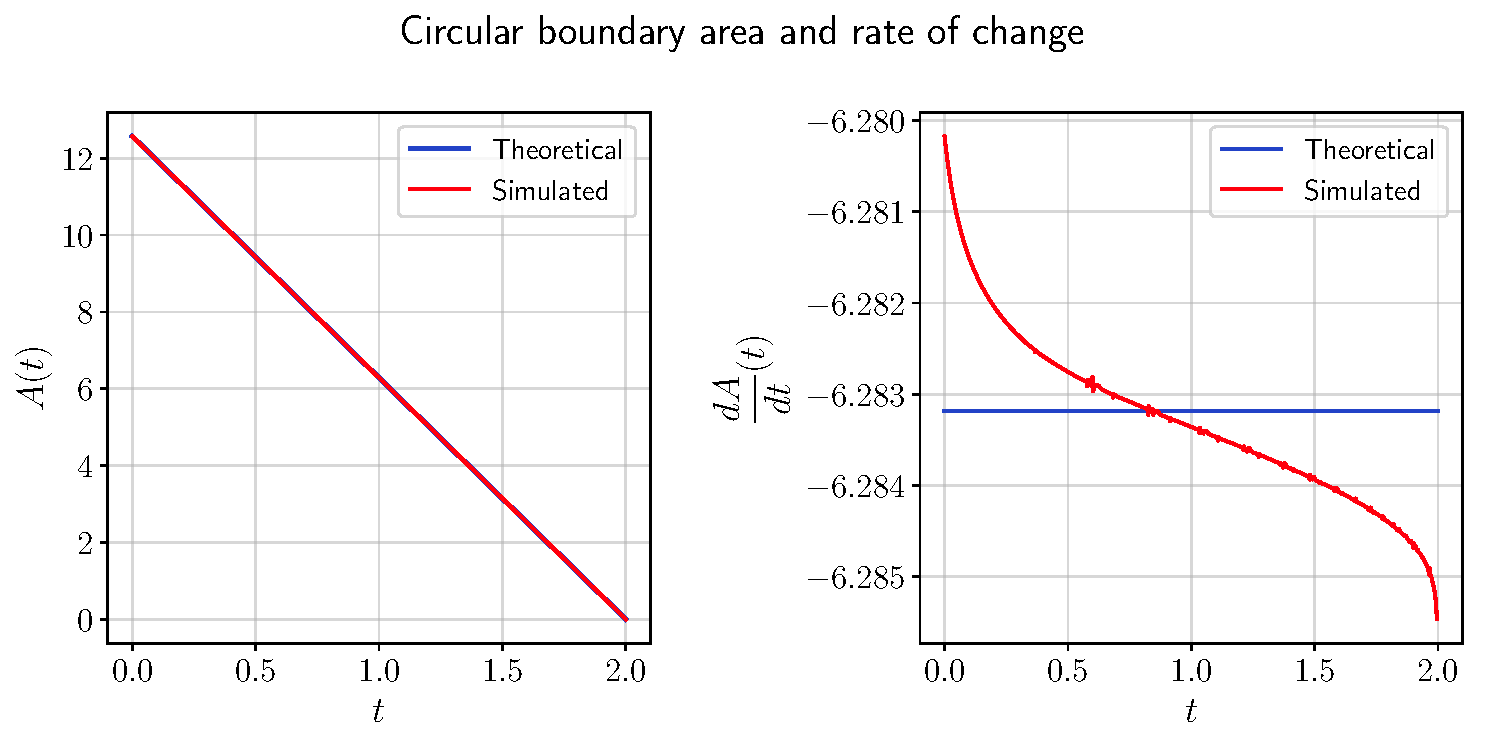
\includegraphics[scale=0.55]{circularboundary_area.pdf}
    \subfloat[\label{fig:area}]{\hspace{.55\linewidth}}
    \subfloat[\label{fig:dAdt}]{\hspace{.45\linewidth}}
    \caption[Circular boundary area and rate of change]{(a) Circle area is in good agreement with the theoretical description. (b) Rate of change is not constant in the numerical simulation, but it is near the theoretical value.}
    \label{fig:circularboundary_area}
\end{figure}

\begin{figure}[t]
    \centering
    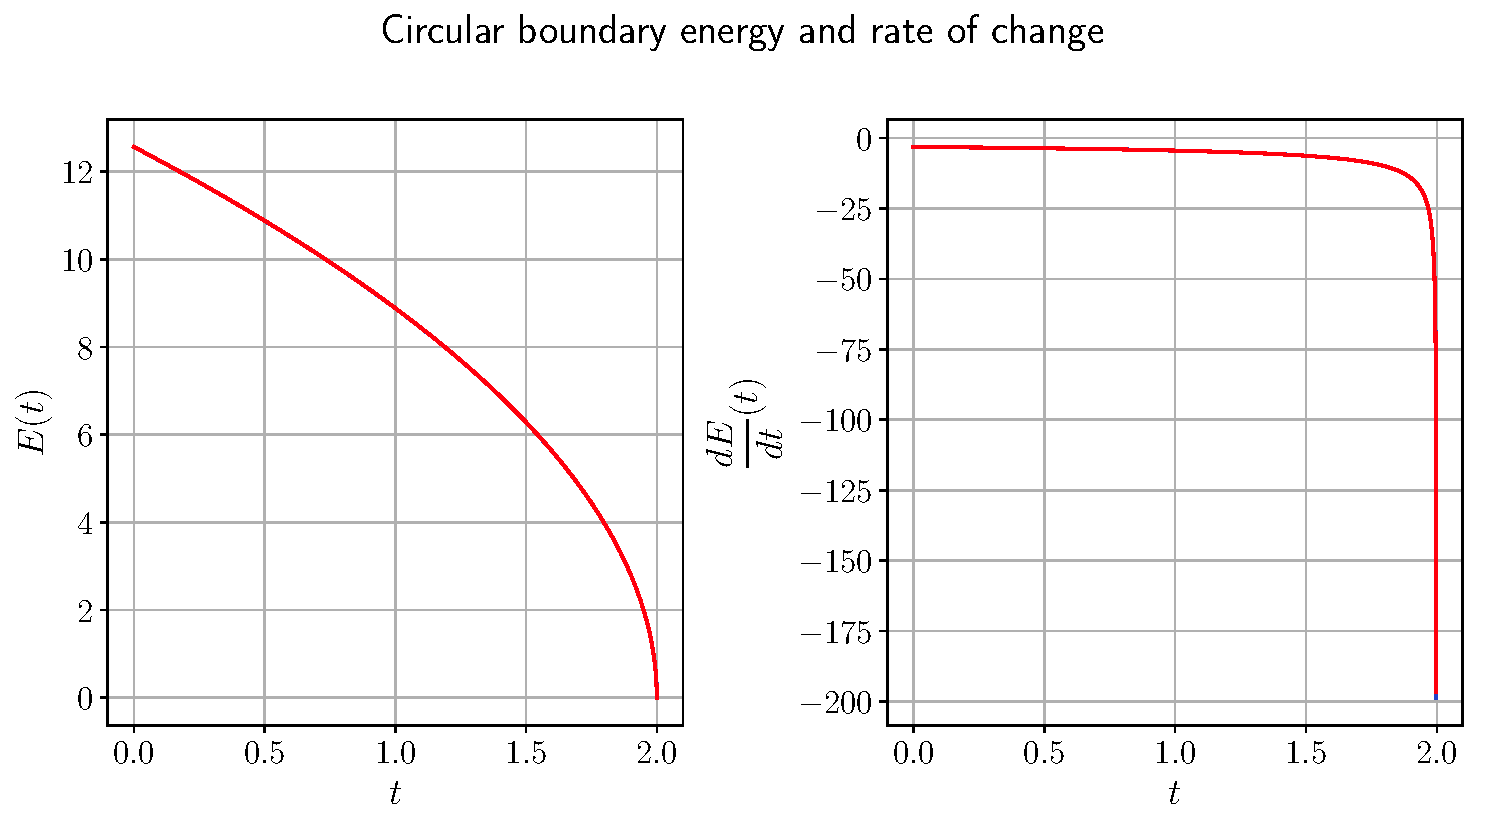
\includegraphics[scale=0.55]{circularboundary_energy.pdf}
    \subfloat[\label{fig:circenergy}]{\hspace{.55\linewidth}}
    \subfloat[\label{fig:circdEdt}]{\hspace{.45\linewidth}}
    \caption[Circular boundary energy and rate of change]{(a) Grain energy function is in good agreement with the evolution of the perimeter of the circle. (b) Rate of change of the energy, in agreement with the precipitation of the boundary motion as the radio goes to zero.}
    \label{fig:circularboundary_energy}
\end{figure}

\subsection{Non-regular Boundary}

Most grains and their boundaries are not restricted to hold circular shapes. The following example shows a boundary described by a polar rose with an initial condition:
\begin{equation*}
    \vxi(s,0) = 3 + \cos(3s)
\end{equation*}
using 14 interpolation points. The number of points is chosen merely to resemble the interpolated function. The simulation is performed using the curvature equations from \eqref{eq:curvaturevelocity}. 

Figure \ref{fig:nonregularboundary} shows the evolution of the polar rose. The equations used ensures energy minimization, which induces that the velocity of the discrete points lying in the concave sections points outside the the rose, trying to achieve some iterations later a fully convex form. In the convex form now the points try to approximate a circle shape, which leads to the known evolution presented in Section \ref{sec:circularboundary}. Figures \ref{fig:nonregularboundary_area} and \ref{fig:nonregularboundary_energy} shows relevant statistics of the experiment. The polar rose area shows qualitatively linear behavior, but a closer look to the derivative shows that there is some perturbation during the minimization, which is soften towards the end of the simulation. The grain boundary energy shows a monotonic decreasing behavior, and its derivative shows a transient where the derivative becomes less negative due to the polar rose correcting its concave parts. After the rose becomes a convex figure, the derivative becomes more and more negative, until numerical collapse at the end of the evolution.

\begin{figure}[t]
    \centering
    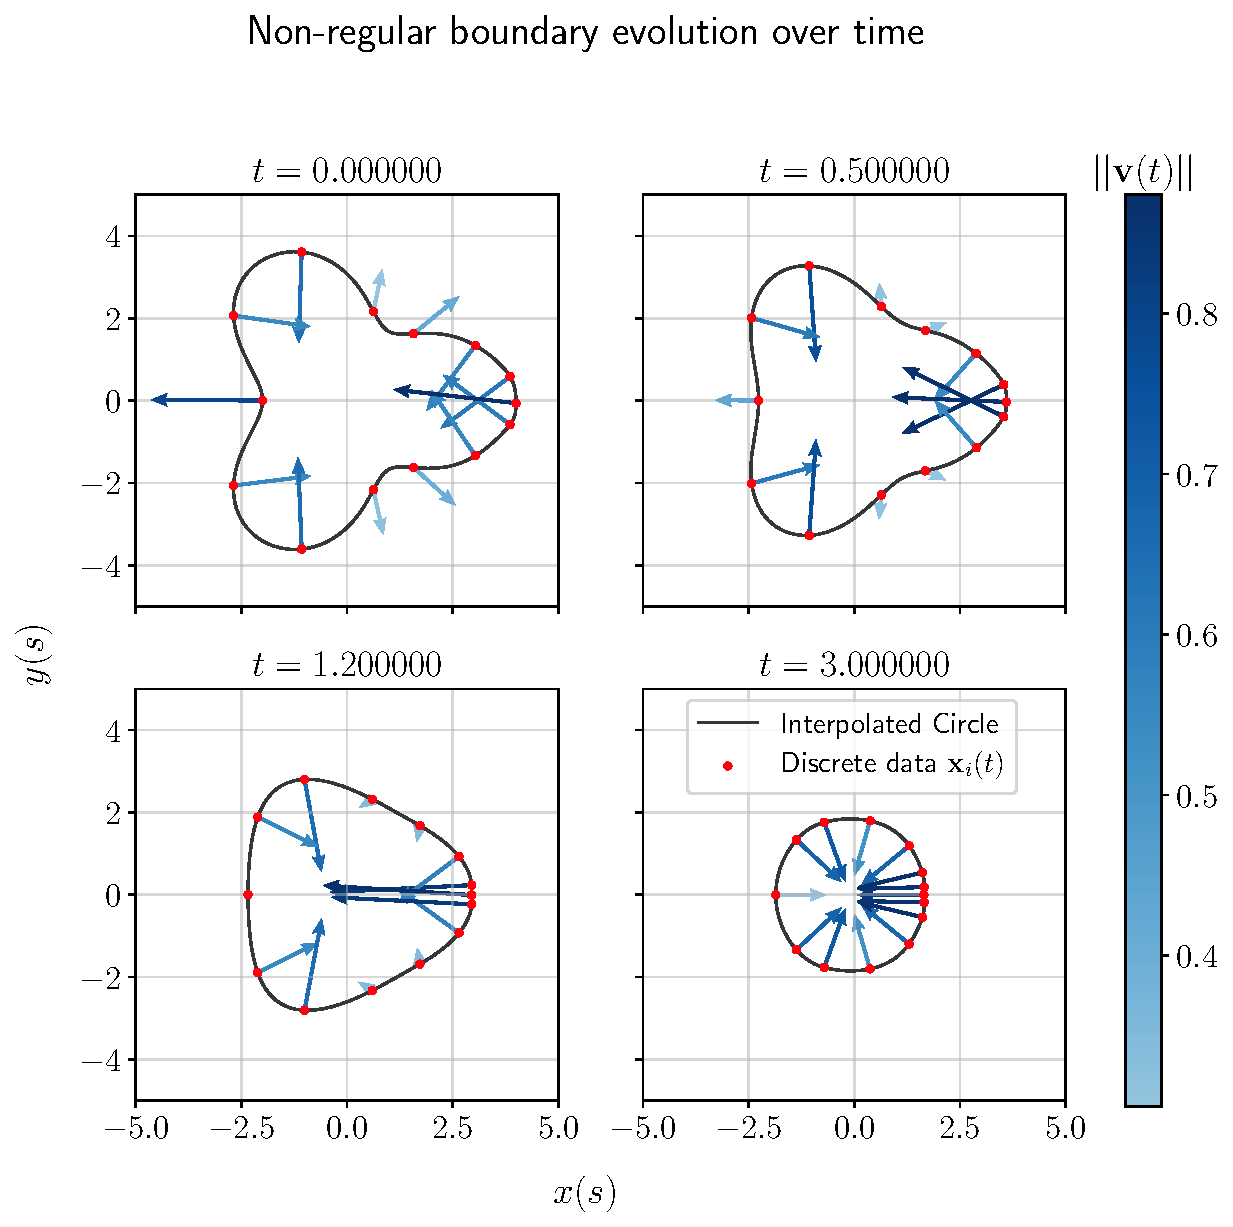
\includegraphics[scale=0.6]{nonregularboundary.pdf}
    \caption[Non-regular boundary evolution]{(Top left) The initial condition at $t=0$ for the polar rose. (Top right) After some time the boundary is driven to correct the curvature while trying to minimize energy. (Bottom left) The boundary is completely convex and all the velocity vectors points to the interior. (Bottom right) The polar rose now has a circle-like shape and the velocity vectors tends to point to the center.}
    \label{fig:nonregularboundary}
\end{figure}



\begin{figure}[t]
    \centering
    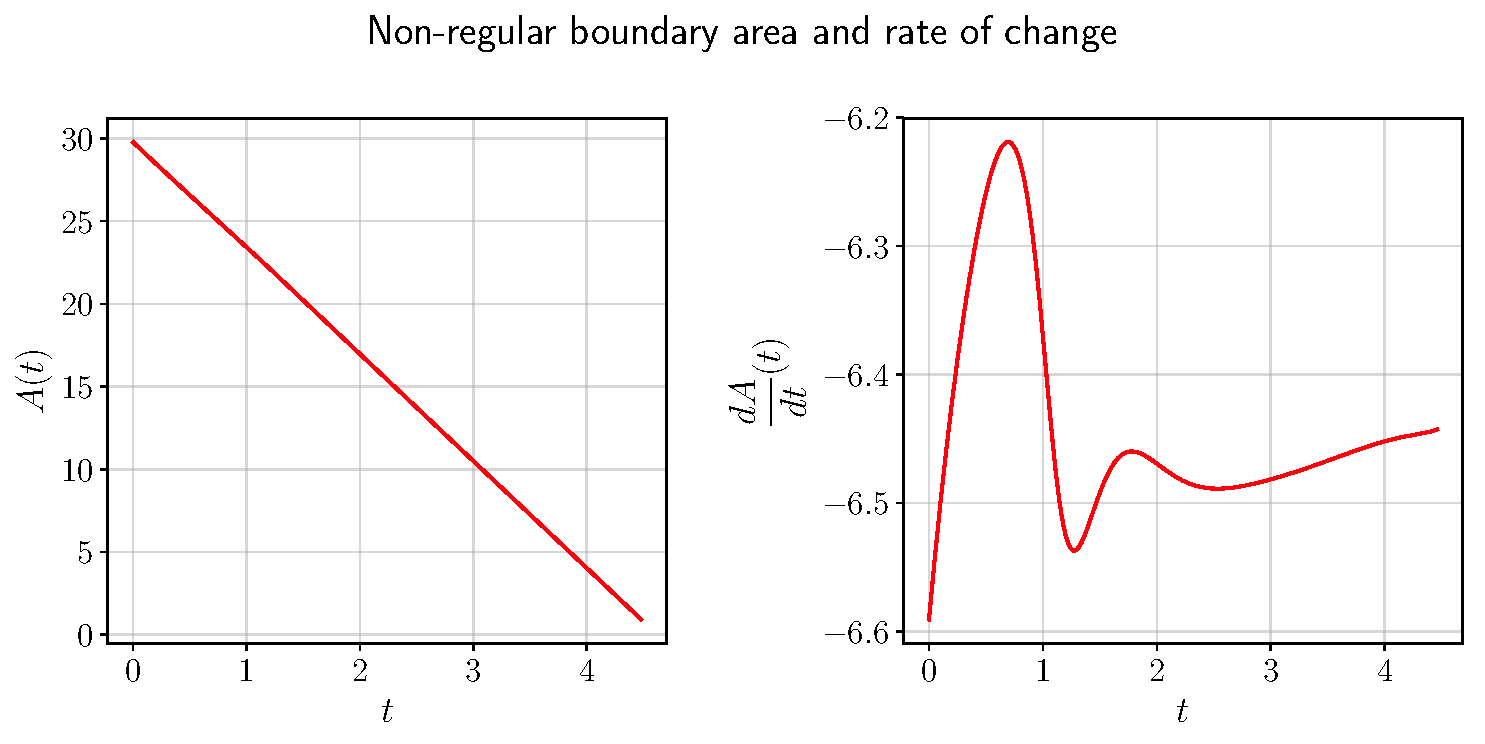
\includegraphics[scale=0.55]{nonregularboundary_area.pdf}
    \subfloat[\label{fig:noncircarea}]{\hspace{.55\linewidth}}
    \subfloat[\label{fig:noncircdAdt}]{\hspace{.45\linewidth}}
    \caption[Non-regular boundary area and rate of change]{(a) Polar rose area shows qualitatively linear behavior, as expected. (b) Rate of change is not constant in the numerical simulation but tries to stabilize.}
    \label{fig:nonregularboundary_area}
\end{figure}

\begin{figure}[t]
    \centering
    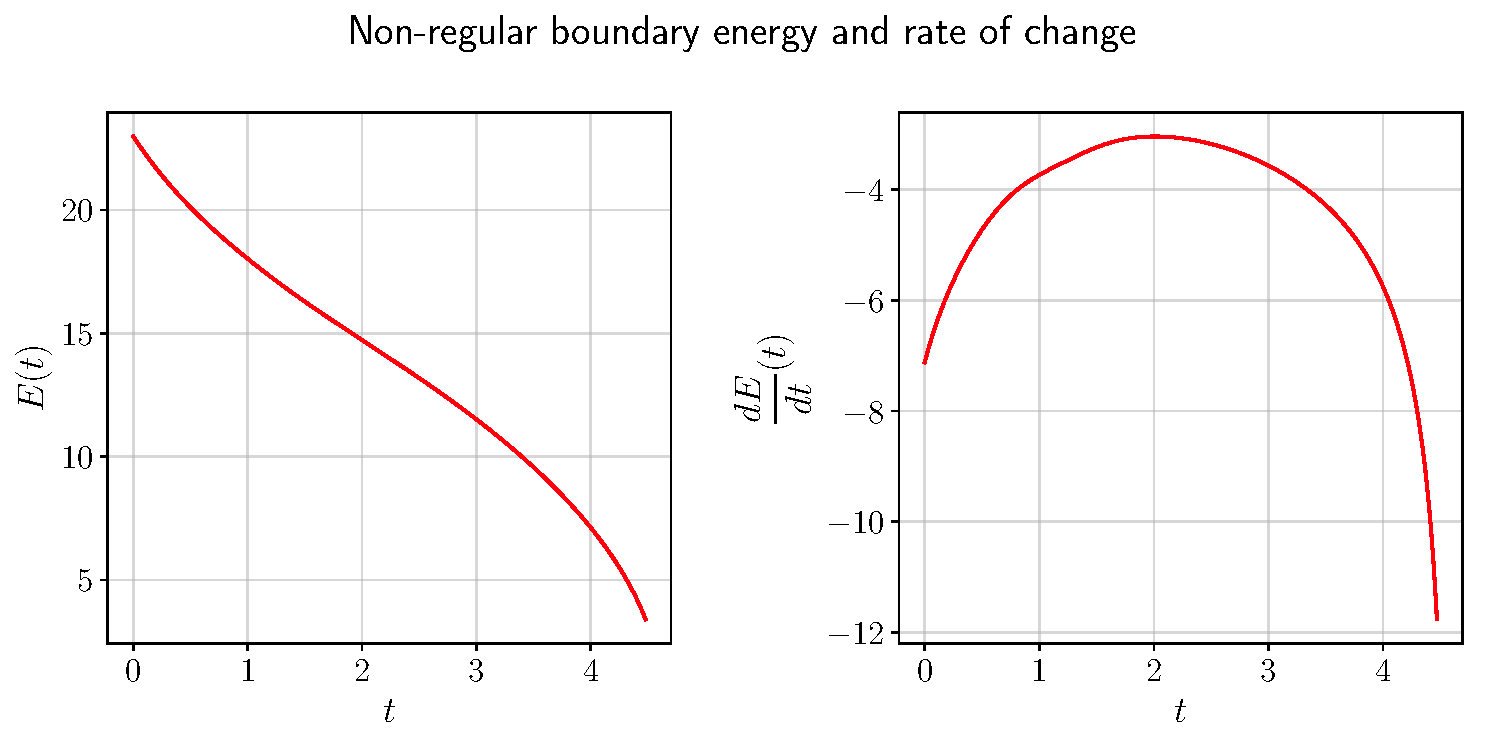
\includegraphics[scale=0.55]{nonregularboundary_energy.pdf}
    \subfloat[\label{fig:noncircenergy}]{\hspace{.55\linewidth}}
    \subfloat[\label{fig:noncircdEdt}]{\hspace{.45\linewidth}}
    \caption[Non-regular boundary energy and rate of change]{(a) Grain energy function shows a monotonic decreasing behavior. (b) Rate of change of the energy collapses at the end of the simulation, meaning that the polar rose is becoming a single point.}
    \label{fig:nonregularboundary_energy}
\end{figure}